\documentclass[xcolor=table]{beamer}
\usepackage{fontspec}
\usepackage{natbib}
\usepackage{gb4e} 
\usepackage[table]{xcolor}
\usepackage{booktabs} 
%\usepackage{color}
\usepackage{graphicx}
\usepackage{bibentry}
\usepackage{tikz}
\usetikzlibrary{trees}
%\usetikzlibrary{mindmap}

% \setmainfont[Mapping=tex-text]{Charis SIL}
\let\sfdefault\rmdefault
%\newcommand{\racine}[1]{\begin{math}\sqrt{#1}\end{math}} 
\newfontfamily\phon[Mapping=tex-text,Ligatures=Common,Scale=MatchLowercase,FakeSlant=0.3]{Charis SIL} 
\newcommand{\ipa}[1]{{\phon \mbox{#1}}} %API tjs en italique
\newcommand{\grise}[1]{\cellcolor{lightgray}\textbf{#1}} 
\newcommand{\ra}{$\Sigma_1$} 
\newcommand{\rc}{$\Sigma_3$} 
\newcommand{\ro}{$\Sigma$} 
\newfontfamily\cn[Mapping=tex-text,Ligatures=Common,Scale=MatchUppercase]{MingLiU}%pour le chinois
\newcommand{\zh}[1]{{\cn #1}}
\newcommand{\rouge}[1]{{\color{red}#1}}
\newcommand{\bleu}[1]{{\color{blue}#1}}
 \begin{document}

 \title{Linguistique panchronique: terrain, formalisation et implémentation}
 \author{Guillaume Jacques}
 \date{}
 \maketitle
 \bibliographystyle{unified}
   \nobibliography{bibliogj.bib}

 
 
    \begin{frame} 
 \frametitle{Plan} 
 
 \begin{itemize}
\item  Recherches précédentes
\item  Programme de recherche
\item  Administration
\end{itemize}
   \end{frame} 
 
 
   \begin{frame} 
 \frametitle{Recherches passées et en cours} 
 
 
  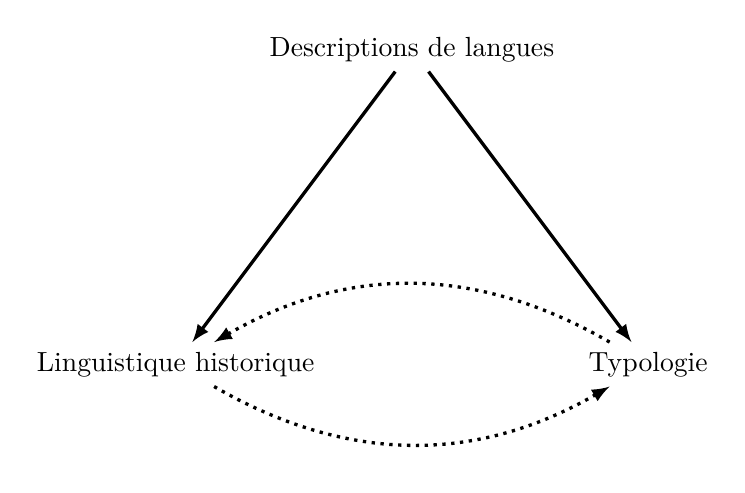
\begin{tikzpicture}
    \node (B) at (0,-1) {Descriptions de langues};
        \node (D) at (-3,-5)  {Linguistique historique};
        \node (G) at (3,-5) {Typologie}; 
 
\tikzstyle{peutetre}=[->,dotted,very thick,>=latex]
\tikzstyle{sur}=[->,very thick,>=latex]
\draw[sur] (B)--(D);
\draw[sur] (B)--(G);
\draw[peutetre] (D)to[bend right](G);
\draw[peutetre] (G)to[bend right](D);
%\draw[peutetre] (D) to[bend right] (H);

\end{tikzpicture} 
 

   \end{frame} 
   
 
   
   \begin{frame} 
 \frametitle{Descriptions de langues} 
  \begin{itemize}
\item Linguistique de terrain (langues à tradition orale)
 \begin{itemize}%[<+->]
 \item rgyalronguique
  \begin{itemize}
\item japhug (Chine, Sichuan, 2002-présent)  
\item zbu (Chine, Sichuan, 2003)
\item situ (Chine, Sichuan, 2012-présent)
\item stau (Chine, Sichuan, 2012-présent)
\end{itemize}
\item pumi (Chine, Sichuan, 2008-2009)
\item tibétain de Tchoné (Chine, Gansu, 2010) 
\item chang naga (Inde du nord-est, 2007)
\item khaling (Népal, Solukhumbu, 2011-présent)
\end{itemize}
\item Langue ancienne
 \begin{itemize}%[<+->]
\item Tangoute
\end{itemize}
\end{itemize}

\end{frame} 
   
      \begin{frame} 
 \frametitle{Linguistique de terrain} 
  \framesubtitle{Japhug} 
    \begin{figure}[H]
\centering
\includegraphics[height=50mm]{carte.JPG}
\end{figure}   
       \end{frame} 
       
      \begin{frame} 
 \frametitle{Linguistique de terrain} 
  \framesubtitle{Japhug} 
 \begin{itemize}%[<+->]
\item Dictionnaire multimédia (juin 2015), projet ANR-corpus HimalCo (2013-2015)
\item \bibentry{jacques10gesar}
\item Corpus de 60h transcrit
\item \bibentry{jacques08}  
\item une dizaine d'articles sur la morphosyntaxe, parus dans \textit{Lingua}, \textit{Linguistic Typology}, \textit{Anthropological Linguistics}, \textit{LTBA}
\end{itemize}
    \end{frame} 
    
      \begin{frame} 
 \frametitle{Linguistique de terrain} 
  \framesubtitle{Khaling} 
  \begin{itemize}%[<+->]
\item Dictionnaire multimédia des verbes (juin 2015)
\item \bibentry{jacques12khaling}  
\item \bibentry{jacques14auditory}
\end{itemize}
    \end{frame} 
    
   \begin{frame} 
 \frametitle{Linguistique historique} 
 
 
  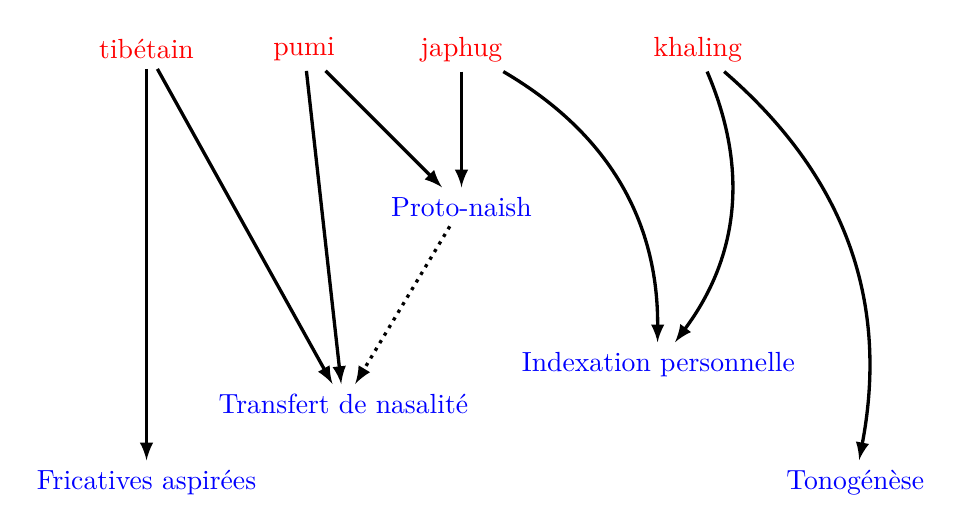
\begin{tikzpicture}
	\node (A) at (4,0) {\rouge{khaling}};
	\node (B) at (1,0) {\rouge{japhug}};
	\node (C) at (-1,0) {\rouge{pumi}};
	\node (D) at (-3,0) {\rouge{tibétain}};
	\node (E) at (1,-2) {\bleu{Proto-naish}};
	\node (F) at (-0.5,-4.5) {\bleu{Transfert de nasalité}};
	\node (G) at (-3,-5.5) {\bleu{Fricatives aspirées}};
	\node (H) at (6,-5.5) {\bleu{Tonogénèse}};
	\node (I) at (3.5,-4) {\bleu{Indexation personnelle}};
%	\node (E) at (-3,0) {\textit{Arapaho}};

		
\tikzstyle{peutetre}=[->,dotted,very thick,>=latex]
\tikzstyle{sur}=[->,very thick,>=latex]
\draw[sur] (A)to[bend left](H);
\draw[sur] (B)--(E);
\draw[sur] (C)--(E);
\draw[sur] (C)--(F);
\draw[sur] (D)--(F);
\draw[sur] (D)--(G);
\draw[sur] (A)to[bend left](I);
\draw[sur] (B)to[bend left](I);
\draw[peutetre] (E)--(F);
%\draw[peutetre] (A)to[bend right](D);
 
%\draw[sur] (G) to[bend left] (F);
\end{tikzpicture}   
 

    \end{frame} 
   \begin{frame} 
 \frametitle{Linguistique historique} 
   \framesubtitle{Publications représentatives} 
 \begin{itemize}%[<+->]
\item \bibentry{jacques.michaud11naish}  
\item \bibentry{jacques11lingua}  
\item \bibentry{jacques13arapaho}  
\end{itemize}
   \end{frame} 
   
   \begin{frame} 
 \frametitle{Typologie} 
 
% Théorie de la grammaticalisation, typologie des marques de voix, du mouvement associé, des systèmes d'indexation polypersonnels

  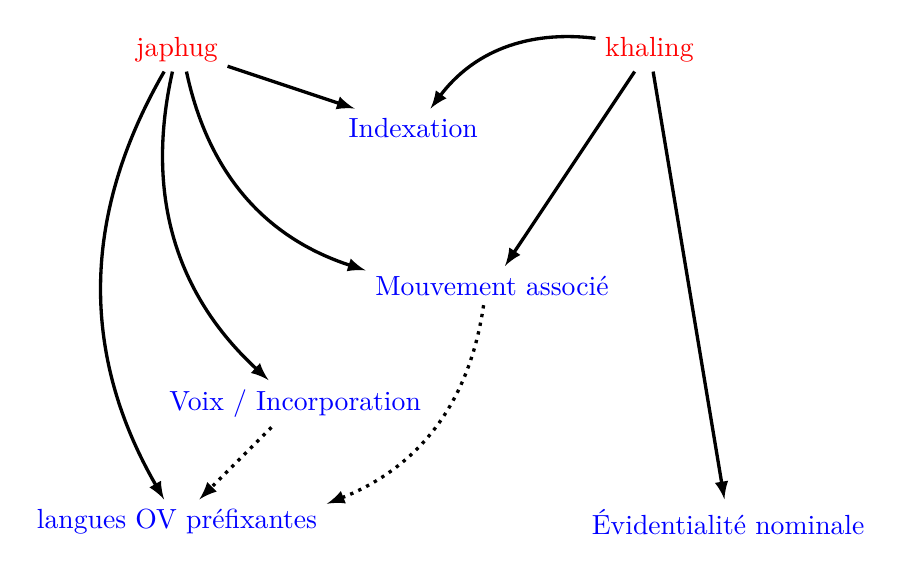
\begin{tikzpicture}
	\node (A) at (3,0) {\rouge{khaling}};
	\node (B) at (-3,0) {\rouge{japhug}};
	\node (C) at (4,-6) {\bleu{Évidentialité nominale}};
	\node (D) at (0,-1) {\bleu{Indexation}};
	\node (E) at (-1.5,-4.5) {\bleu{Voix / Incorporation}};
	\node (F) at (-3,-6) {\bleu{langues OV préfixantes}};
	\node (G) at (1,-3) {\bleu{Mouvement associé}};
\tikzstyle{peutetre}=[->,dotted,very thick,>=latex]
\tikzstyle{sur}=[->,very thick,>=latex]
\draw[sur] (A)--(C);
\draw[sur] (A)to[bend right](D);
\draw[sur] (A)--(G);
\draw[sur] (B)--(D);
\draw[sur] (B) to[bend right](G);
\draw[sur] (B) to[bend right] (E);
\draw[sur] (B) to[bend right] (F);
\draw[peutetre] (E)--(F);
\draw[peutetre] (G) to[bend left] (F);
\end{tikzpicture}  
   \end{frame}  
   
    \begin{frame} 
 \frametitle{Typologie} 
  \framesubtitle{Publications représentatives} 
 \begin{itemize}%[<+->]
\item \bibentry{jacques12incorp}  
\item \bibentry{jacques13harmonization}  
\item \bibentry{jacques14antipassive}  
\item \bibentry{antonov14need}  
\end{itemize}
   \end{frame} 
    
  \begin{frame} 
 \frametitle{Projet de recherche} 
 
  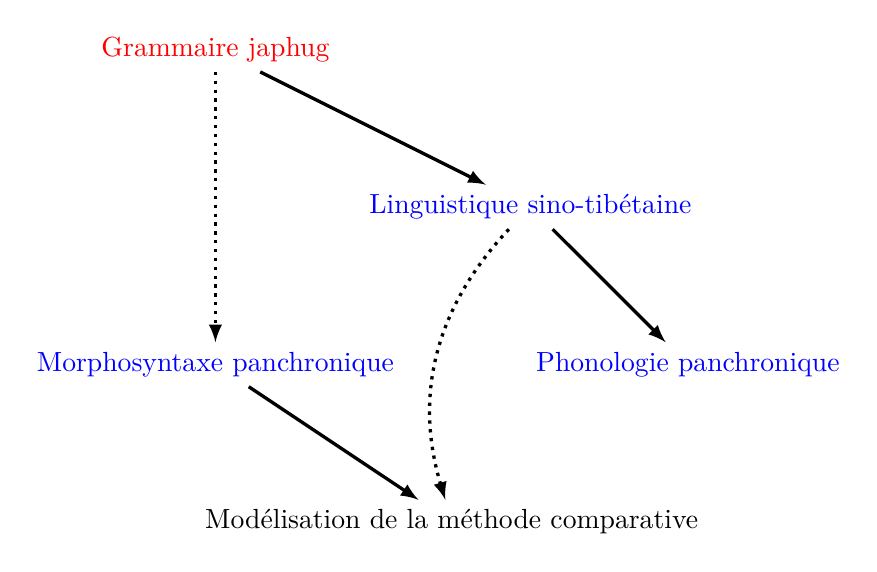
\begin{tikzpicture}
    \node (B) at (-3,-1) {\rouge{Grammaire japhug}};
        \node (D) at (1,-3)  {\bleu{Linguistique sino-tibétaine}};
       \node (F) at (3,-5)  {\bleu{Phonologie panchronique}};%\\ Adversative};
        \node (G) at (-3,-5) {\bleu{Morphosyntaxe panchronique}}; 
             \node (H) at (0,-7)  {Modélisation de la méthode comparative};
\tikzstyle{peutetre}=[->,dotted,very thick,>=latex]
\tikzstyle{sur}=[->,very thick,>=latex]
\draw[sur] (B)--(D);
\draw[sur] (D)--(F);
\draw[sur] (G)--(H);
\draw[peutetre] (B)--(G);
\draw[peutetre] (D) to[bend right] (H);

\end{tikzpicture}

   
  \end{frame}   

   \begin{frame} 
 \frametitle{Grammaire Japhug} 
 \begin{itemize}%[<+->]
 \item 2015-2016: publication d'une dizaine d'articles
\item 2017-2019: rédaction de la grammaire
\end{itemize}
   \end{frame} 
   
   \begin{frame} 
 \frametitle{Linguistique comparative des langues sino-tibétaines} 

 
  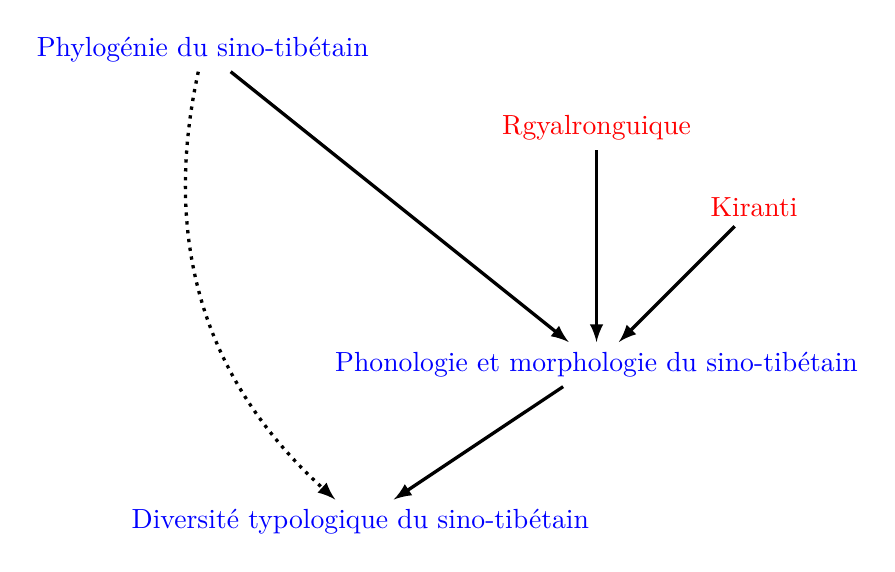
\begin{tikzpicture}
    \node (A) at (-3,0) {\bleu{Phylogénie du sino-tibétain}};
     \node (B) at (2,-1) {\rouge{Rgyalronguique}};
     \node (C) at (4,-2) {\rouge{Kiranti}};
        \node (D) at (2,-4)  {\bleu{Phonologie et morphologie du sino-tibétain}};
        \node (E) at (-1,-6)  {\bleu{Diversité typologique du sino-tibétain}};

\tikzstyle{peutetre}=[->,dotted,very thick,>=latex]
\tikzstyle{sur}=[->,very thick,>=latex]
\draw[sur] (A)--(D);
\draw[sur] (B)--(D);
\draw[sur] (C)--(D);
\draw[sur] (D)--(E);
\draw[peutetre] (A) to[bend right] (E);

\end{tikzpicture} 
 
   \end{frame} 

   \begin{frame} 
 \frametitle{Linguistique comparative des langues sino-tibétaines} 
 
Publications principales des doctorants qui travaillent sous ma direction:
\begin{itemize}
\item  \bibentry{lai13fuyin}
\item  \bibentry{gongxun14agreement}  
\item  \bibentry{lai14person}
\end{itemize}   
   \end{frame} 

%   \begin{frame} 
% \frametitle{Phonologie panchronique} 
% \begin{itemize}%[<+->]
% \item Unidirectionnalité des changements phonétiques
% \item Changements de lieu d'articulation dans les systèmes consonantiques
%\end{itemize}
%   \end{frame} 


   \begin{frame} 
 \frametitle{Modélisation de la méthode comparative} 
 \begin{itemize}%[<+->]
 \item  Implémentation en transducteurs à état fini des changements phonétiques
  \item Application de la \textit{minimal description length} en morphologie et en linguistique pour mesurer la complexité relative d'hypothèses concurrentes
  \item Modélisation de l'analogie
\end{itemize}
   \end{frame} 
   
   \begin{frame} 
 \frametitle{Animation de la recherche et enseignement} 
 \begin{itemize}%[<+->]
 \item  Directeur de l'équipe  `Linguistique descriptive des langues d’Asie, phonologie, morphosyntaxe et comparatisme' du CRLAO.
\item Responsabilités éditoriales
    \begin{itemize}%[<+->]
\item  co-directeur: \textit{Cahiers de linguistique d'Asie orientale} (Brill, 2013--)
\item  `area editor': \textit{Linguistic Vanguard} (Mouton de Gruyter, 2015--)
\item membre du comité éditorial: \textit{Diachronica}, \textit{Linguistics of the Tibeto-Burman Area}
\end{itemize}
 \item  Projets ANR
  \begin{itemize}%[<+->]
 \item  Pasqi (2007-2013 CRLAO, LACITO)
  \item Himalco (2013-2015 CRLAO, LACITO, HTL, MICA), coordinateur
\end{itemize}
 \item  Archive Pangloss (LACITO, CNRS)
  \item Labex EFL, axe 6 (ressources)
\end{itemize}
   \end{frame} 

 
\begin{frame} 
\frametitle{Animation de la recherche et enseignement} 
   \begin{itemize}%[<+->]
\item Cours de M1 (INALCO-Paris III), de typologie, 24h
\item Direction ou co-direction de 4 doctorants.
 \end{itemize}
\end{frame} 
 
 \begin{frame} 
 \frametitle{Publications additionnelles}

   \small
\begin{itemize}
\item  \bibentry{jacques14ergative}  
\item  \bibentry{jacques15sr}  
\item  \bibentry{jacques15causative}
\item  \bibentry{jacques15spontaneous}
\item  \bibentry{jacques15derivational.khaling}
\end{itemize}
 \end{frame}
\end{document}